%----------------------------------------------------------------------------------------
%	PACKAGES AND THEMES
%----------------------------------------------------------------------------------------
\documentclass[aspectratio=169,xcolor=dvipsnames, t]{beamer}
\usepackage{fontspec} % Allows using custom font. MUST be before loading the theme!
\usetheme{SimplePlusAIC}
\usepackage{hyperref}
\usepackage{graphicx} % Allows including images
\usepackage{booktabs} % Allows the use of \toprule, \midrule and  \bottomrule in tables
\usepackage{svg} %allows using svg figures
\usepackage{tikz}
\usepackage{makecell}
\usepackage{wrapfig}
\usepackage{algorithm}
\usepackage{algorithmic}
\usepackage[style=ieee]{biblatex}
\addbibresource{ref.bib}

% ADD YOUR PACKAGES BELOW

%----------------------------------------------------------------------------------------
%	TITLE PAGE CONFIGURATION
%----------------------------------------------------------------------------------------

\title[Parareal Algorithm]{Parareal Algorithm: An Advanced Analysis}
\subtitle{Internship Presentation}

\author[O. BOUHENNICHE]{Oussama BOUHENNICHE \\[2mm]{\small Supervisors: M. Christophe PRUD’HOMME}}

\institute[]{University of Strasbourg\\[1mm]{\small Cemosis}}

\date{\today} % Date, can be changed to a custom date
%----------------------------------------------------------------------------------------
%	PRESENTATION SLIDES
%----------------------------------------------------------------------------------------

\begin{document}

\maketitlepage

\begin{frame}[t]{Overview}
    \tableofcontents
\end{frame}

%------------------------------------------------
% Section divider frame
\makesection{Introduction}

%------------------------------------------------
% Bullets
\begin{frame}{Context}
    \begin{itemize}
        \item Solving time-dependent ordinary differential equations (ODEs) numerically is crucial in computational fields.
        \item Traditional methods can be highly time-consuming, especially for long simulations or intricate systems.
    \end{itemize}
\begin{block}{}
    The Parareal algorithm \footfullcite{lions2001resolution} a parallel-in-time integration method designed to efficiently solve time-dependent differential equations
\end{block}
\end{frame}

%------------------------------------------------
% Lists
\begin{frame}{Objectives}
    \begin{enumerate}
        \item Analyzing the convergence of the Parareal algorithm by evaluating the number of iterations required for different solver combinations
        \item Investigate how the order of convergence of the Parareal algorithm varies with different solvers
        \item Evaluating the performance of the Parareal algorithm in relation to the number of processes used
    \end{enumerate}
\end{frame}

%------------------------------------------------
% Section divider frame
\makesection{Background}

%------------------------------------------------
\begin{frame}{Parareal Algorithm 1/3}
    \begin{block}{}
    Developed by Lions, Maday, and Turinici in 2001, It aims to solve problems of the form:
    $$
    \frac{du}{dt} = f(t,u) \;\;\;,\; u(t_0) = u_0
    $$
    \begin{itemize}
        \item Accelerates time-dependent ODE solving using parallel computing.
        \item Decomposes the time domain into smaller intervals that can be processed simultaneously.
    \end{itemize}
\end{block}
\end{frame}

\begin{frame}{Parareal Algorithm 2/3}

\begin{itemize}
    \item \textbf{How it Works}
    \begin{itemize}
        \item Combines coarse and fine propagators.
        \item Iteratively corrects the coarse solution with fine solution details.
    \end{itemize}
    \item \textbf{Parallelization}
    \begin{itemize}
        \item Distributes computation across multiple processors.
        \item Significantly reduces computation time for large-scale problems.
    \end{itemize}
\end{itemize}
    
\end{frame}

\begin{frame}{Parareal Algorithm 3/3}
    \begin{algorithm}[H]
\caption{Parareal Algorithm (parallel)} 
\begin{algorithmic}[1]
\STATE \textbf{Given:} Coarse function $G$, fine function $F$, number of time steps $N$, maximum number of iterations $K$, $\epsilon$ tolerance, number of process.
\STATE \textbf{Initialize: in sequential} \begin{itemize}
    \item  $U_0^0 = u_0; \;\;\;\; U_{j+1}^0 = G(t_j,t_{j+1}, U_j^0) \;\;\;j = 0,1, \ldots, N-1$
\end{itemize}
\WHILE{$|U^k-U^{k-1}| > \epsilon $}
    \begin{itemize}
        \item run the fine solver on each process and given a sub-interval of the time slices, in parallel: $F(t_j,t_{j+1}, U_j^{k-1}) \;\;\;\;\;\;\;\;\;\; j = 0,1, ... ,N-1$.
        \item  communicate fine solution and update u in sequetial and share it to all process: $ U_{j+1}^k = G(t_j,t_{j+1},U_j^k) + F(t_j,t_{j+1},U_j^{k-1}) -G(t_j,t_{j+1},U_j^{k-1})$.  
    \end{itemize}
\ENDWHILE
\STATE \textbf{Return:} $U^k$
\end{algorithmic}
\end{algorithm}
\end{frame}

%------------------------------------------------
% Section divider frame
\makesection{Methodology and Implementation}

%------------------------------------------------
\begin{frame}{Previous Works}
    \begin{block}{\textbf{Python Package for Parareal Algorithm}}
        \begin{itemize}
            \item \textbf{Foundation:} Developed a Python package for solving time-dependent differential equations using the Parareal algorithm.
            \item \textbf{Core Features:}
                \begin{itemize}
                    \item \textbf{Solver Integration:} Supports multiple ODE solvers (explicit/implicit Euler, Runge-Kutta, SciPy solvers).
                    \item \textbf{Parallelization:} Utilizes Python's multiprocessing and MPI for parallel execution.
                    \item \textbf{Customization:} Allows user-defined solvers, adjustable time intervals, convergence criteria, and maximum iterations.
                \end{itemize}
        \end{itemize}
    \end{block}
\end{frame}

\begin{frame}{Experimental Setup 1/2}
    \begin{itemize}
        \item \textbf{Parallel Environment}
        \begin{itemize}
            \item Tests conducted on a high-performance computing system with multiple cores (Gaya)
            
        \end{itemize}
        \item \textbf{ Solver Configurations}
        \newline
        The study involved a variety of solvers to cover a broad range of explicit and implicit methods:
        \begin{itemize}
            \item \textbf{Explicit Solvers:}
            \begin{itemize}
                \item Explicit Euler
                \item Explicit RK2
                \item Explicit RK4
            \end{itemize}
            \item \textbf{Implicit Solvers:}
            \begin{itemize}
                \item Implicit Euler
                \item Implicit RK2
                \item Implicit RK4
            \end{itemize}
        \end{itemize}

    \end{itemize}
\end{frame}

\begin{frame}{Experimental Setup 2/2}
\begin{itemize}
    \item \textbf{Test Systems:}
    \begin{itemize}
        \item \textbf{Lorenz system \footfullcite{lorenz1963deterministic}}
        $$
        \begin{cases}
        \displaystyle\frac{dx}{dt} = \sigma(y - x) \\
        \displaystyle\frac{dy}{dt} = x(\rho - z) - y \\
        \displaystyle\frac{dz}{dt} = xy - \beta z
        \end{cases}
        $$
        \item \textbf{System 1:}
        $
            \frac{dy}{dt} = -ty^2
        $
        \item \textbf{System 2:}
        $
            \frac{dy}{dt} = -y+ cos(t)
        $
        \item \textbf{System 3:}
        $
            \frac{dy}{dt} = -2y
        $
    \end{itemize}
\end{itemize}
    
\end{frame}

\begin{frame}{Tests Setup 1/2}
    \begin{block}{\textbf{Number of Parareal Iterations and Convergence Order Tests}}
        \begin{itemize}
            \item \textbf{Tested on 3 systems}
            \item \textbf{Solvers Used}: Explicit/Implicit (Euler, RK2, RK4).
            \item \textbf{Initial Setup}: 
                \begin{itemize}
                    \item Initial conditions set as specified.
                    \item Time span $[0, 5]$ discretized.
                \end{itemize}
            \item \textbf{Execution}: Recorded number of Parareal iterations to reach tolerance.
            \item \textbf{Convergence Order $P$ Calculation}:
                \[
                P = \frac{1}{n} \sum_{i=0}^{n-1} \frac{\log\left(\frac{e_{i+1}}{e_i}\right)}{\log\left(\frac{\Delta_{i+1}}{\Delta_i}\right)}
                \]
        \end{itemize}
    \end{block}
\end{frame}

\begin{frame}{Tests Setup 2/2}
    \begin{block}{\textbf{Execution Time and Speedup Tests}}
        \begin{itemize}
            \item \textbf{System Tested}: Lorenz system.
            \item \textbf{Solvers Used}: Explicit/Implicit (Euler, RK2, RK4).
            \item \textbf{Initial Setup}: 
                \begin{itemize}
                    \item Initial conditions set as specified.
                    \item Time span $[0, 10]$ discretized.
                \end{itemize}
            \item \textbf{Parallel Execution}: 
                \begin{itemize}
                    \item Used up to 128 processes with MPI.
                    \item Recorded execution times $T_P$.
                \end{itemize}
            \item \textbf{Speedup $S$ Calculation}:
                \[
                S = \frac{T_1}{T_P}
                \]
        \end{itemize}
    \end{block}
\end{frame}

\begin{frame}{Parallel Test Execution}
    \begin{itemize}
            \item \textbf{Parallel Testing:} Shell scripts created to run tests in parallel, significantly reducing execution time.
            \item \textbf{Automation:} 
                \begin{itemize}
                    \item Automates test execution using parallel processing.
                    \item Handles large test suites efficiently.
                \end{itemize}
            \item \textbf{Test Configuration:} Defines test parameters, file names, and configurations.
            \item \textbf{Test Execution:} Executes tests by calling Python scripts with necessary arguments.
            \item \textbf{Result Handling:} Saves results and cleans up temporary files.
        \end{itemize}
\end{frame}


%------------------------------------------------
% Section divider frame
\makesection{Results and Analysis}

%------------------------------------------------

\begin{frame}{Number of Parareal Iterations for Convergence}
    \begin{columns}
\begin{column}{0.33\textwidth}
   \begin{figure}[ht!]
    \centering
    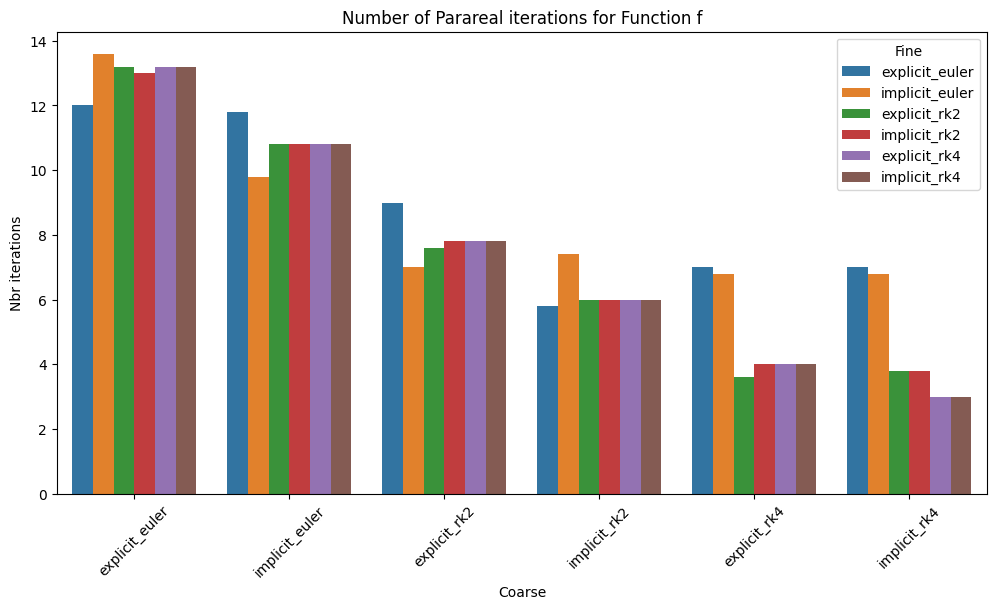
\includegraphics[width=0.9\textwidth]{figures/nbr_iter_f.png}
    \caption{Number of Parareal iterations for system 1}
    \label{fig:4}
\end{figure}
\end{column}
\begin{column}{0.33\textwidth}  %%<--- here
    \begin{center}
     \begin{figure}[H]
    \centering
    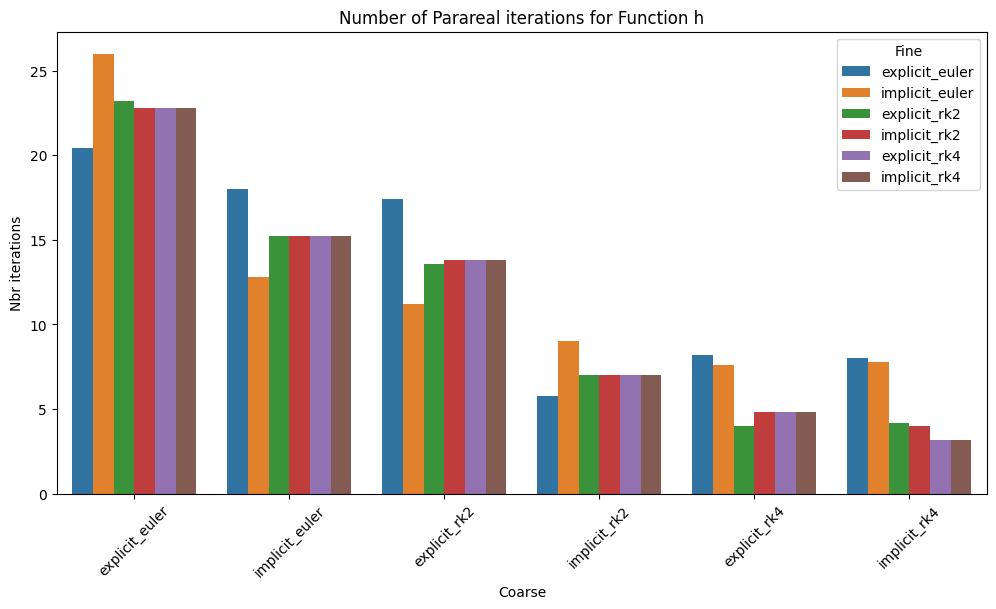
\includegraphics[width=.85\textwidth]{figures/nbr_iter_h.png}
    \caption{Number of Parareal iterations for system 2}
    \label{fig:8}
\end{figure}
     \end{center}
\end{column}
\begin{column}{0.33\textwidth}  %%<--- here
    \begin{center}
     \begin{figure}[H]
    \centering
    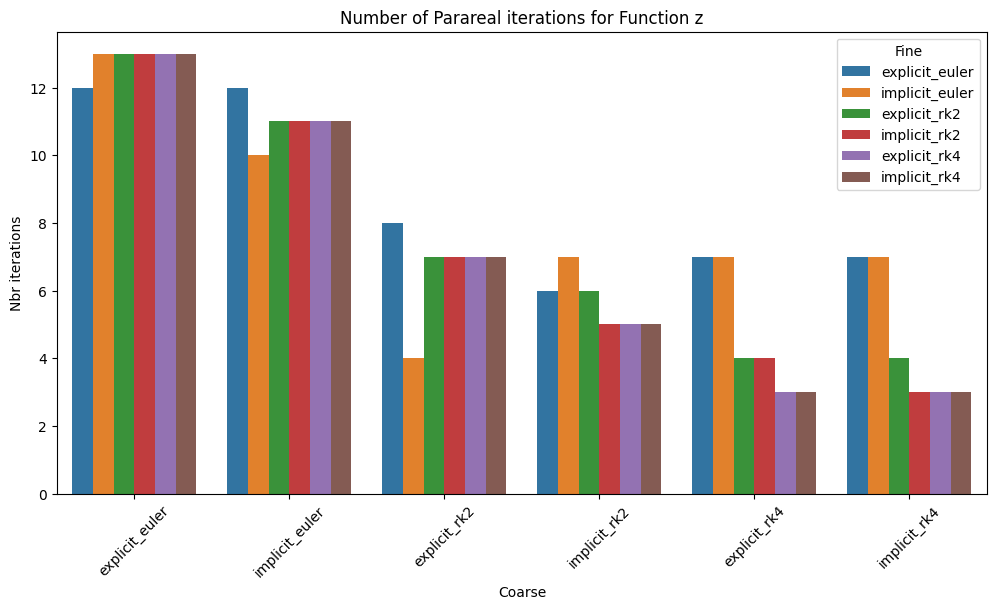
\includegraphics[width=.85\textwidth]{figures/nbr_iter_z.png}
    \caption{Number of Parareal iterations for system 3}
    \label{fig:8}
\end{figure}
     \end{center}
\end{column}
\end{columns}
\begin{itemize}
    \item The number of iterations required for convergence is significantly influenced by the choice of coarse solver
    \item Higher-order coarse solvers lead to faster convergence
\end{itemize}
\end{frame}

\begin{frame}{Order of Convergence}
    \begin{columns}
\begin{column}{0.33\textwidth}
   \begin{figure}[ht!]
    \centering
    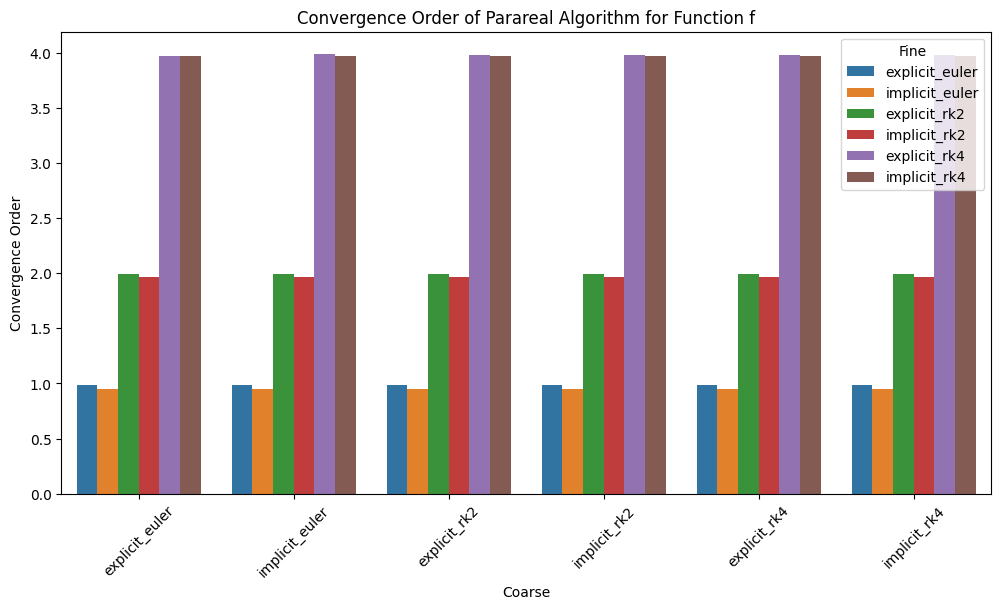
\includegraphics[width=0.9\textwidth]{figures/cv_ord_f.png}
    \caption{Convergence Order of Parareal Algorithm for system 1}
    \label{fig:4}
\end{figure}
\end{column}
\begin{column}{0.33\textwidth}  %%<--- here
    \begin{center}
     \begin{figure}[H]
    \centering
    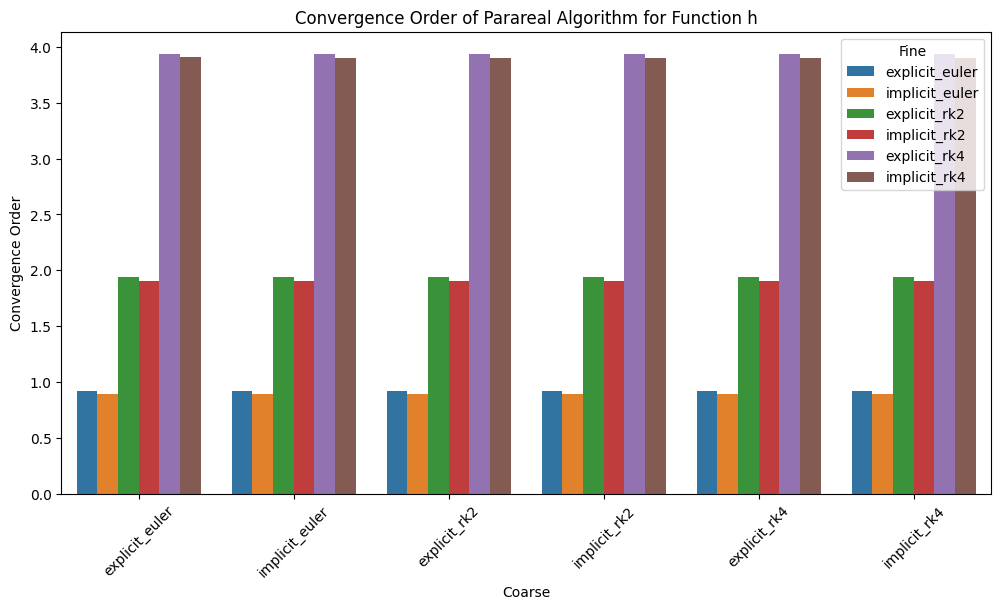
\includegraphics[width=.85\textwidth]{figures/cv_ord_h.png}
    \caption{Convergence Order of Parareal Algorithm for system 2}
    \label{fig:8}
\end{figure}
     \end{center}
\end{column}
\begin{column}{0.33\textwidth}  %%<--- here
    \begin{center}
     \begin{figure}[H]
    \centering
    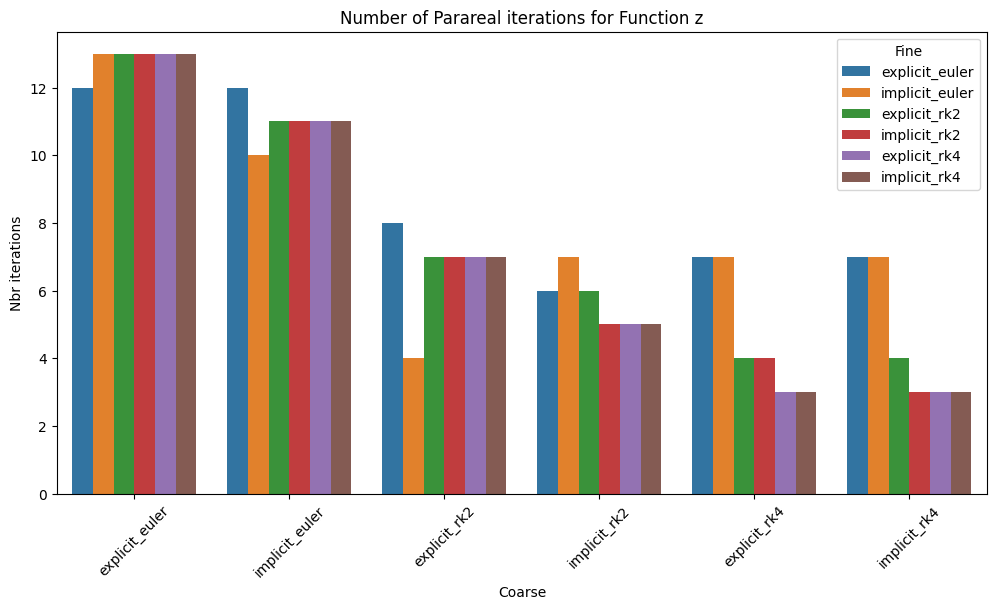
\includegraphics[width=.85\textwidth]{figures/nbr_iter_z.png}
    \caption{Convergence Order of Parareal Algorithm for system 3}
    \label{fig:8}
\end{figure}
     \end{center}
\end{column}
\end{columns}
\begin{itemize}
    \item The fine solver dictates the overall convergence order of the Parareal algorithm
    \item Higher-order fine solvers enhance accuracy and improve the convergence rate
\end{itemize}
\end{frame}

\begin{frame}{Execution Time and Speedup}
    \begin{columns}
\begin{column}{0.45\textwidth}
   \begin{figure}[ht!]
    \centering
    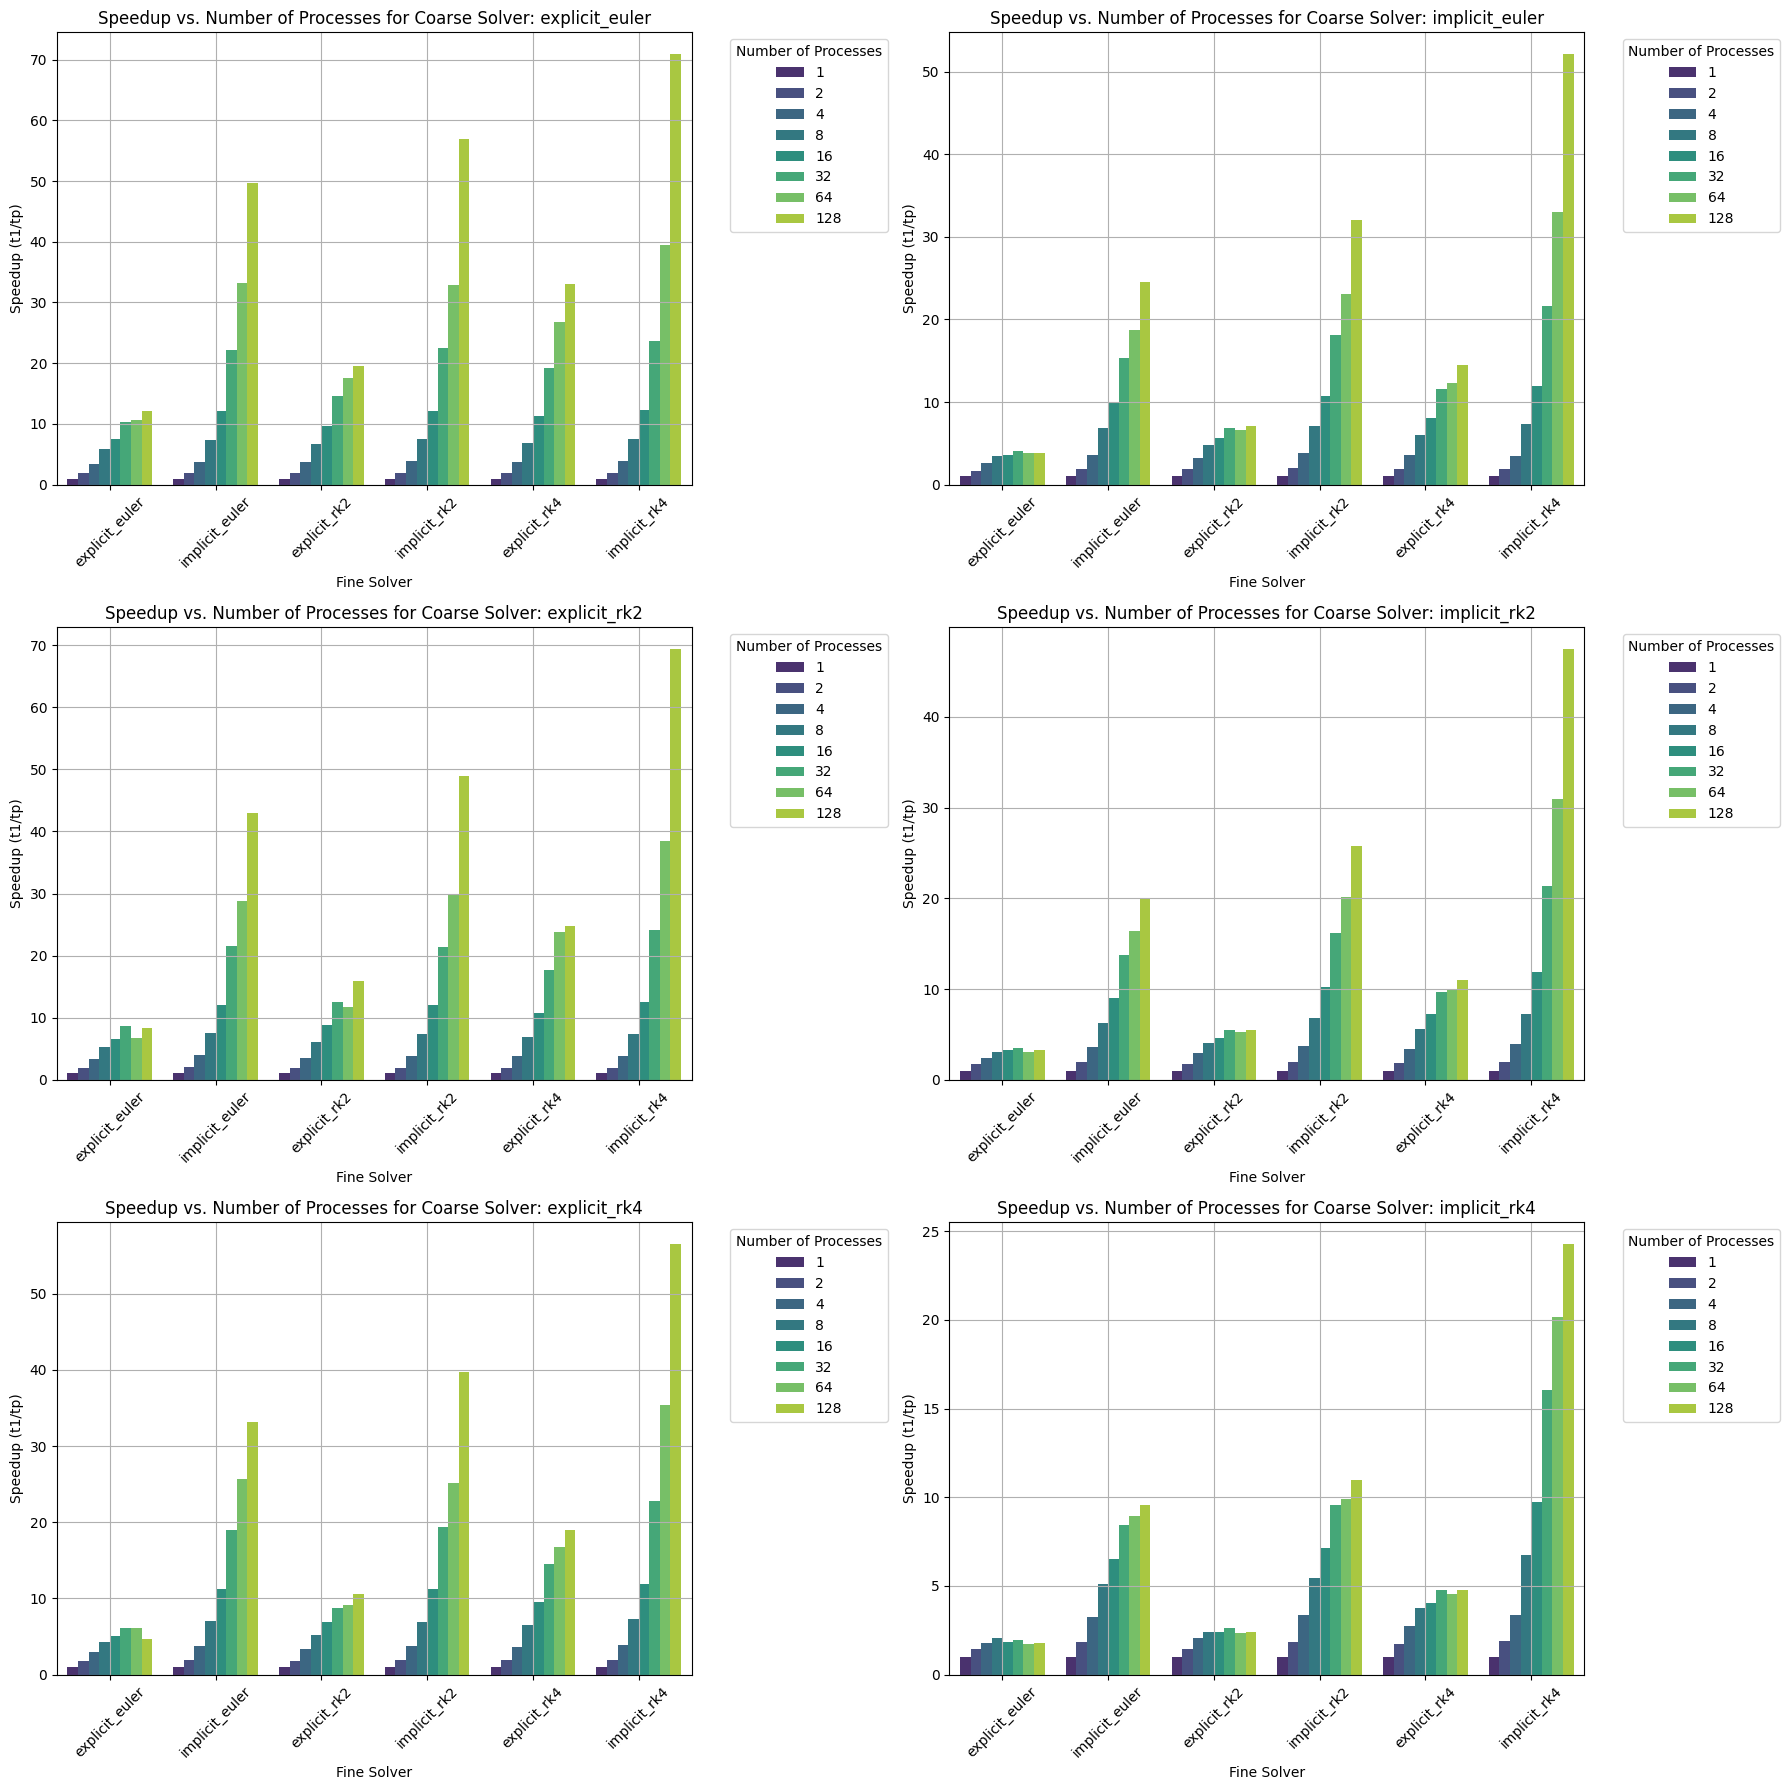
\includegraphics[width=.7\textwidth]{figures/perf.png}
    \caption{Speedup vs. Number of Processes for Different solvers combination}
    \label{fig:4}
\end{figure}
\end{column}
\begin{column}{0.55\textwidth}
    \begin{itemize}
        \item Parallel execution greatly reduces time, showing near-linear speedup with fewer processes
        \item  Speedup decreases with more processes, especially for explicit solvers, due to communication overhead
    \end{itemize}
\end{column}
\end{columns}
\end{frame}


% Section divider frame
\makesection{Conclusion}
\begin{frame}{Conclusion}
    \begin{block}{\textbf{Key Findings}}
        \begin{itemize}
            \item \textbf{Convergence Analysis:} 
                \begin{itemize}
                    \item Higher-order coarse solvers lead to faster convergence.
                \end{itemize}
            \item \textbf{Order of Convergence:} 
                \begin{itemize}
                    \item Fine solver dictates convergence order.
                    \item Higher-order fine solvers improve accuracy and rate.
                \end{itemize}
            \item \textbf{Performance Evaluation:} 
                \begin{itemize}
                    \item Parallel execution reduces time, with near-linear speedup initially.
                    \item Diminishing returns with more processes due to communication overhead.
                \end{itemize}
        \end{itemize}
    \end{block}
    
    \textbf{Future Prospects:}
    \begin{itemize}
    \item Further exploration with Parareal for PDEs using frameworks like feel++.
    \end{itemize}
\end{frame}
%------------------------------------------------
% Refenrenced
\begin{frame}[allowframebreaks]{References}
    %\nocite{*}
    \printbibliography
	
\end{frame}

%----------------------------------------------------------------------------------------
% Final PAGE
% Set the text that is showed on the final slide
\finalpagetext{Thank you for your attention}
%----------------------------------------------------------------------------------------
\makefinalpage
%----------------------------------------------------------------------------------------
\end{document}